\documentclass[1p]{elsarticle_modified}
%\bibliographystyle{elsarticle-num}

%\usepackage[colorlinks]{hyperref}
%\usepackage{abbrmath_seonhwa} %\Abb, \Ascr, \Acal ,\Abf, \Afrak
\usepackage{amsfonts}
\usepackage{amssymb}
\usepackage{amsmath}
\usepackage{amsthm}
\usepackage{scalefnt}
\usepackage{amsbsy}
\usepackage{kotex}
\usepackage{caption}
\usepackage{subfig}
\usepackage{color}
\usepackage{graphicx}
\usepackage{xcolor} %% white, black, red, green, blue, cyan, magenta, yellow
\usepackage{float}
\usepackage{setspace}
\usepackage{hyperref}

\usepackage{tikz}
\usetikzlibrary{arrows}

\usepackage{multirow}
\usepackage{array} % fixed length table
\usepackage{hhline}

%%%%%%%%%%%%%%%%%%%%%
\makeatletter
\renewcommand*\env@matrix[1][\arraystretch]{%
	\edef\arraystretch{#1}%
	\hskip -\arraycolsep
	\let\@ifnextchar\new@ifnextchar
	\array{*\c@MaxMatrixCols c}}
\makeatother %https://tex.stackexchange.com/questions/14071/how-can-i-increase-the-line-spacing-in-a-matrix
%%%%%%%%%%%%%%%

\usepackage[normalem]{ulem}

\newcommand{\msout}[1]{\ifmmode\text{\sout{\ensuremath{#1}}}\else\sout{#1}\fi}
%SOURCE: \msout is \stkout macro in https://tex.stackexchange.com/questions/20609/strikeout-in-math-mode

\newcommand{\cancel}[1]{
	\ifmmode
	{\color{red}\msout{#1}}
	\else
	{\color{red}\sout{#1}}
	\fi
}

\newcommand{\add}[1]{
	{\color{blue}\uwave{#1}}
}

\newcommand{\replace}[2]{
	\ifmmode
	{\color{red}\msout{#1}}{\color{blue}\uwave{#2}}
	\else
	{\color{red}\sout{#1}}{\color{blue}\uwave{#2}}
	\fi
}

\newcommand{\Sol}{\mathcal{S}} %segment
\newcommand{\D}{D} %diagram
\newcommand{\A}{\mathcal{A}} %arc


%%%%%%%%%%%%%%%%%%%%%%%%%%%%%5 test

\def\sl{\operatorname{\textup{SL}}(2,\Cbb)}
\def\psl{\operatorname{\textup{PSL}}(2,\Cbb)}
\def\quan{\mkern 1mu \triangleright \mkern 1mu}

\theoremstyle{definition}
\newtheorem{thm}{Theorem}[section]
\newtheorem{prop}[thm]{Proposition}
\newtheorem{lem}[thm]{Lemma}
\newtheorem{ques}[thm]{Question}
\newtheorem{cor}[thm]{Corollary}
\newtheorem{defn}[thm]{Definition}
\newtheorem{exam}[thm]{Example}
\newtheorem{rmk}[thm]{Remark}
\newtheorem{alg}[thm]{Algorithm}

\newcommand{\I}{\sqrt{-1}}
\begin{document}

%\begin{frontmatter}
%
%\title{Boundary parabolic representations of knots up to 8 crossings}
%
%%% Group authors per affiliation:
%\author{Yunhi Cho} 
%\address{Department of Mathematics, University of Seoul, Seoul, Korea}
%\ead{yhcho@uos.ac.kr}
%
%
%\author{Seonhwa Kim} %\fnref{s_kim}}
%\address{Center for Geometry and Physics, Institute for Basic Science, Pohang, 37673, Korea}
%\ead{ryeona17@ibs.re.kr}
%
%\author{Hyuk Kim}
%\address{Department of Mathematical Sciences, Seoul National University, Seoul 08826, Korea}
%\ead{hyukkim@snu.ac.kr}
%
%\author{Seokbeom Yoon}
%\address{Department of Mathematical Sciences, Seoul National University, Seoul, 08826,  Korea}
%\ead{sbyoon15@snu.ac.kr}
%
%\begin{abstract}
%We find all boundary parabolic representation of knots up to 8 crossings.
%
%\end{abstract}
%\begin{keyword}
%    \MSC[2010] 57M25 
%\end{keyword}
%
%\end{frontmatter}

%\linenumbers
%\tableofcontents
%
\newcommand\colored[1]{\textcolor{white}{\rule[-0.35ex]{0.8em}{1.4ex}}\kern-0.8em\color{red} #1}%
%\newcommand\colored[1]{\textcolor{white}{ #1}\kern-2.17ex	\textcolor{white}{ #1}\kern-1.81ex	\textcolor{white}{ #1}\kern-2.15ex\color{red}#1	}

{\Large $\underline{12n_{0649}~(K12n_{0649})}$}

\setlength{\tabcolsep}{10pt}
\renewcommand{\arraystretch}{1.6}
\vspace{1cm}\begin{tabular}{m{100pt}>{\centering\arraybackslash}m{274pt}}
\multirow{5}{120pt}{
	\centering
	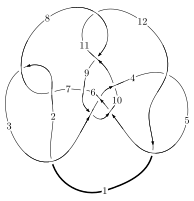
\includegraphics[width=112pt]{../../../GIT/diagram.site/Diagrams/png/2738_12n_0649.png}\\
\ \ \ A knot diagram\footnotemark}&
\allowdisplaybreaks
\textbf{Linearized knot diagam} \\
\cline{2-2}
 &
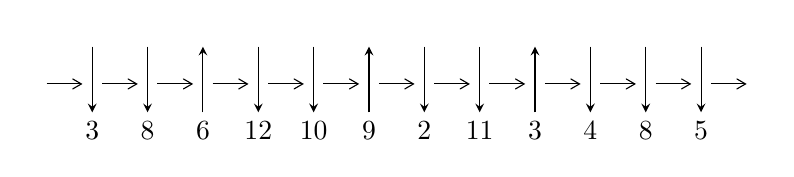
\begin{tikzpicture}[x=20pt, y=17pt]
	% nodes
	\node (C0) at (0, 0) {};
	\node (C1) at (1, 0) {};
	\node (C1U) at (1, +1) {};
	\node (C1D) at (1, -1) {3};

	\node (C2) at (2, 0) {};
	\node (C2U) at (2, +1) {};
	\node (C2D) at (2, -1) {8};

	\node (C3) at (3, 0) {};
	\node (C3U) at (3, +1) {};
	\node (C3D) at (3, -1) {6};

	\node (C4) at (4, 0) {};
	\node (C4U) at (4, +1) {};
	\node (C4D) at (4, -1) {12};

	\node (C5) at (5, 0) {};
	\node (C5U) at (5, +1) {};
	\node (C5D) at (5, -1) {10};

	\node (C6) at (6, 0) {};
	\node (C6U) at (6, +1) {};
	\node (C6D) at (6, -1) {9};

	\node (C7) at (7, 0) {};
	\node (C7U) at (7, +1) {};
	\node (C7D) at (7, -1) {2};

	\node (C8) at (8, 0) {};
	\node (C8U) at (8, +1) {};
	\node (C8D) at (8, -1) {11};

	\node (C9) at (9, 0) {};
	\node (C9U) at (9, +1) {};
	\node (C9D) at (9, -1) {3};

	\node (C10) at (10, 0) {};
	\node (C10U) at (10, +1) {};
	\node (C10D) at (10, -1) {4};

	\node (C11) at (11, 0) {};
	\node (C11U) at (11, +1) {};
	\node (C11D) at (11, -1) {8};

	\node (C12) at (12, 0) {};
	\node (C12U) at (12, +1) {};
	\node (C12D) at (12, -1) {5};
	\node (C13) at (13, 0) {};

	% arrows
	\draw[->,>={angle 60}]
	(C0) edge (C1) (C1) edge (C2) (C2) edge (C3) (C3) edge (C4) (C4) edge (C5) (C5) edge (C6) (C6) edge (C7) (C7) edge (C8) (C8) edge (C9) (C9) edge (C10) (C10) edge (C11) (C11) edge (C12) (C12) edge (C13) ;	\draw[->,>=stealth]
	(C1U) edge (C1D) (C2U) edge (C2D) (C3D) edge (C3U) (C4U) edge (C4D) (C5U) edge (C5D) (C6D) edge (C6U) (C7U) edge (C7D) (C8U) edge (C8D) (C9D) edge (C9U) (C10U) edge (C10D) (C11U) edge (C11D) (C12U) edge (C12D) ;
	\end{tikzpicture} \\
\hhline{~~} \\& 
\textbf{Solving Sequence} \\ \cline{2-2} 
 &
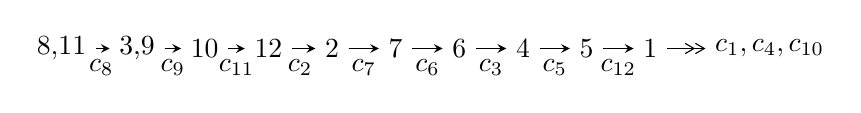
\begin{tikzpicture}[x=23pt, y=7pt]
	% node
	\node (A0) at (-1/8, 0) {8,11};
	\node (A1) at (17/16, 0) {3,9};
	\node (A2) at (17/8, 0) {10};
	\node (A3) at (25/8, 0) {12};
	\node (A4) at (33/8, 0) {2};
	\node (A5) at (41/8, 0) {7};
	\node (A6) at (49/8, 0) {6};
	\node (A7) at (57/8, 0) {4};
	\node (A8) at (65/8, 0) {5};
	\node (A9) at (73/8, 0) {1};
	\node (C1) at (1/2, -1) {$c_{8}$};
	\node (C2) at (13/8, -1) {$c_{9}$};
	\node (C3) at (21/8, -1) {$c_{11}$};
	\node (C4) at (29/8, -1) {$c_{2}$};
	\node (C5) at (37/8, -1) {$c_{7}$};
	\node (C6) at (45/8, -1) {$c_{6}$};
	\node (C7) at (53/8, -1) {$c_{3}$};
	\node (C8) at (61/8, -1) {$c_{5}$};
	\node (C9) at (69/8, -1) {$c_{12}$};
	\node (A10) at (11, 0) {$c_{1},c_{4},c_{10}$};

	% edge
	\draw[->,>=stealth]	
	(A0) edge (A1) (A1) edge (A2) (A2) edge (A3) (A3) edge (A4) (A4) edge (A5) (A5) edge (A6) (A6) edge (A7) (A7) edge (A8) (A8) edge (A9) ;
	\draw[->>,>={angle 60}]	
	(A9) edge (A10);
\end{tikzpicture} \\ 

\end{tabular} \\

\footnotetext{
The image of knot diagram is generated by the software ``\textbf{Draw programme}" developed by Andrew Bartholomew(\url{http://www.layer8.co.uk/maths/draw/index.htm\#Running-draw}), where we modified some parts for our purpose(\url{https://github.com/CATsTAILs/LinksPainter}).
}\phantom \\ \newline 
\centering \textbf{Ideals for irreducible components\footnotemark of $X_{\text{par}}$} 
 
\begin{align*}
I^u_{1}&=\langle 
3.75673\times10^{194} u^{68}-1.58940\times10^{195} u^{67}+\cdots+9.63648\times10^{193} b-1.53579\times10^{195},\\
\phantom{I^u_{1}}&\phantom{= \langle  }1.26586\times10^{195} u^{68}-5.38237\times10^{195} u^{67}+\cdots+9.63648\times10^{193} a-5.24849\times10^{195},\;u^{69}-4 u^{68}+\cdots-8 u-1\rangle \\
I^u_{2}&=\langle 
6.02923\times10^{18} u^{30}-1.34813\times10^{20} u^{29}+\cdots+4.00441\times10^{19} b-6.44459\times10^{19},\\
\phantom{I^u_{2}}&\phantom{= \langle  }1.49489\times10^{20} u^{30}-1.48284\times10^{21} u^{29}+\cdots+4.00441\times10^{19} a+2.33807\times10^{19},\;u^{31}-11 u^{30}+\cdots+u+1\rangle \\
\\
\end{align*}
\raggedright * 2 irreducible components of $\dim_{\mathbb{C}}=0$, with total 100 representations.\\
\footnotetext{All coefficients of polynomials are rational numbers. But the coefficients are sometimes approximated in decimal forms when there is not enough margin.}
\newpage
\renewcommand{\arraystretch}{1}
\centering \section*{I. $I^u_{1}= \langle 3.76\times10^{194} u^{68}-1.59\times10^{195} u^{67}+\cdots+9.64\times10^{193} b-1.54\times10^{195},\;1.27\times10^{195} u^{68}-5.38\times10^{195} u^{67}+\cdots+9.64\times10^{193} a-5.25\times10^{195},\;u^{69}-4 u^{68}+\cdots-8 u-1 \rangle$}
\flushleft \textbf{(i) Arc colorings}\\
\begin{tabular}{m{7pt} m{180pt} m{7pt} m{180pt} }
\flushright $a_{8}=$&$\begin{pmatrix}1\\0\end{pmatrix}$ \\
\flushright $a_{11}=$&$\begin{pmatrix}0\\u\end{pmatrix}$ \\
\flushright $a_{3}=$&$\begin{pmatrix}-13.1361 u^{68}+55.8541 u^{67}+\cdots+202.166 u+54.4648\\-3.89844 u^{68}+16.4936 u^{67}+\cdots+59.7728 u+15.9372\end{pmatrix}$ \\
\flushright $a_{9}=$&$\begin{pmatrix}1\\u^2\end{pmatrix}$ \\
\flushright $a_{10}=$&$\begin{pmatrix}10.3030 u^{68}-43.5171 u^{67}+\cdots-162.149 u-44.5391\\2.44719 u^{68}-10.4597 u^{67}+\cdots-42.5909 u-11.6937\end{pmatrix}$ \\
\flushright $a_{12}=$&$\begin{pmatrix}- u\\u\end{pmatrix}$ \\
\flushright $a_{2}=$&$\begin{pmatrix}-17.0346 u^{68}+72.3477 u^{67}+\cdots+261.938 u+70.4021\\-3.89844 u^{68}+16.4936 u^{67}+\cdots+59.7728 u+15.9372\end{pmatrix}$ \\
\flushright $a_{7}=$&$\begin{pmatrix}12.2442 u^{68}-51.2281 u^{67}+\cdots-204.361 u-61.3466\\2.63447 u^{68}-11.1419 u^{67}+\cdots-46.1582 u-13.3409\end{pmatrix}$ \\
\flushright $a_{6}=$&$\begin{pmatrix}9.89356 u^{68}-41.1837 u^{67}+\cdots-163.968 u-50.2569\\2.47796 u^{68}-10.4551 u^{67}+\cdots-43.3750 u-12.6991\end{pmatrix}$ \\
\flushright $a_{4}=$&$\begin{pmatrix}-13.5371 u^{68}+57.7238 u^{67}+\cdots+204.879 u+52.8631\\-3.08045 u^{68}+13.1709 u^{67}+\cdots+54.5833 u+13.6099\end{pmatrix}$ \\
\flushright $a_{5}=$&$\begin{pmatrix}-12.3892 u^{68}+52.8068 u^{67}+\cdots+186.100 u+48.4386\\-4.22829 u^{68}+18.0878 u^{67}+\cdots+73.3622 u+18.0344\end{pmatrix}$ \\
\flushright $a_{1}=$&$\begin{pmatrix}-11.8031 u^{68}+49.9636 u^{67}+\cdots+191.753 u+52.5886\\-4.36464 u^{68}+18.3517 u^{67}+\cdots+53.8331 u+17.0568\end{pmatrix}$\\&\end{tabular}
\flushleft \textbf{(ii) Obstruction class $= -1$}\\~\\
\flushleft \textbf{(iii) Cusp Shapes $= 8.83213 u^{68}-38.7205 u^{67}+\cdots-158.969 u-40.1796$}\\~\\
\newpage\renewcommand{\arraystretch}{1}
\flushleft \textbf{(iv) u-Polynomials at the component}\newline \\
\begin{tabular}{m{50pt}|m{274pt}}
Crossings & \hspace{64pt}u-Polynomials at each crossing \\
\hline $$\begin{aligned}c_{1}\end{aligned}$$&$\begin{aligned}
&u^{69}+93 u^{68}+\cdots+5452015640 u+242020249
\end{aligned}$\\
\hline $$\begin{aligned}c_{2},c_{7}\end{aligned}$$&$\begin{aligned}
&u^{69}- u^{68}+\cdots+173530 u-15557
\end{aligned}$\\
\hline $$\begin{aligned}c_{3}\end{aligned}$$&$\begin{aligned}
&u^{69}+5 u^{68}+\cdots+20 u-1
\end{aligned}$\\
\hline $$\begin{aligned}c_{4},c_{12}\end{aligned}$$&$\begin{aligned}
&u^{69}+2 u^{68}+\cdots-27 u-1
\end{aligned}$\\
\hline $$\begin{aligned}c_{5}\end{aligned}$$&$\begin{aligned}
&u^{69}+4 u^{68}+\cdots-28636 u+15839
\end{aligned}$\\
\hline $$\begin{aligned}c_{6}\end{aligned}$$&$\begin{aligned}
&u^{69}+15 u^{68}+\cdots+1134199439 u+510193511
\end{aligned}$\\
\hline $$\begin{aligned}c_{8},c_{11}\end{aligned}$$&$\begin{aligned}
&u^{69}+4 u^{68}+\cdots-8 u+1
\end{aligned}$\\
\hline $$\begin{aligned}c_{9}\end{aligned}$$&$\begin{aligned}
&u^{69}+2 u^{68}+\cdots-137905545 u-27775009
\end{aligned}$\\
\hline $$\begin{aligned}c_{10}\end{aligned}$$&$\begin{aligned}
&u^{69}-14 u^{67}+\cdots-40553 u+9503
\end{aligned}$\\
\hline
\end{tabular}\\~\\
\newpage\renewcommand{\arraystretch}{1}
\flushleft \textbf{(v) Riley Polynomials at the component}\newline \\
\begin{tabular}{m{50pt}|m{274pt}}
Crossings & \hspace{64pt}Riley Polynomials at each crossing \\
\hline $$\begin{aligned}c_{1}\end{aligned}$$&$\begin{aligned}
&y^{69}-229 y^{68}+\cdots-1.55\times10^{19} y-5.86\times10^{16}
\end{aligned}$\\
\hline $$\begin{aligned}c_{2},c_{7}\end{aligned}$$&$\begin{aligned}
&y^{69}-93 y^{68}+\cdots+5452015640 y-242020249
\end{aligned}$\\
\hline $$\begin{aligned}c_{3}\end{aligned}$$&$\begin{aligned}
&y^{69}-3 y^{68}+\cdots+574 y-1
\end{aligned}$\\
\hline $$\begin{aligned}c_{4},c_{12}\end{aligned}$$&$\begin{aligned}
&y^{69}-64 y^{68}+\cdots-109 y-1
\end{aligned}$\\
\hline $$\begin{aligned}c_{5}\end{aligned}$$&$\begin{aligned}
&y^{69}-24 y^{68}+\cdots+7028148224 y-250873921
\end{aligned}$\\
\hline $$\begin{aligned}c_{6}\end{aligned}$$&$\begin{aligned}
&y^{69}+41 y^{68}+\cdots-3357290919353259237 y-260297418666507121
\end{aligned}$\\
\hline $$\begin{aligned}c_{8},c_{11}\end{aligned}$$&$\begin{aligned}
&y^{69}+8 y^{68}+\cdots+40 y-1
\end{aligned}$\\
\hline $$\begin{aligned}c_{9}\end{aligned}$$&$\begin{aligned}
&y^{69}+40 y^{68}+\cdots-1503105609784333 y-771451124950081
\end{aligned}$\\
\hline $$\begin{aligned}c_{10}\end{aligned}$$&$\begin{aligned}
&y^{69}-28 y^{68}+\cdots+2430025777 y-90307009
\end{aligned}$\\
\hline
\end{tabular}\\~\\
\newpage\flushleft \textbf{(vi) Complex Volumes and Cusp Shapes}
$$\begin{array}{c|c|c}  
\text{Solutions to }I^u_{1}& \I (\text{vol} + \sqrt{-1}CS) & \text{Cusp shape}\\
 \hline 
\begin{aligned}
u &= \phantom{-}0.620567 + 0.768614 I \\
a &= \phantom{-}0.295115 + 1.061520 I \\
b &= -0.266968 - 0.592280 I\end{aligned}
 & -0.27963 - 2.36978 I & \phantom{-0.000000 } 0 \\ \hline\begin{aligned}
u &= \phantom{-}0.620567 - 0.768614 I \\
a &= \phantom{-}0.295115 - 1.061520 I \\
b &= -0.266968 + 0.592280 I\end{aligned}
 & -0.27963 + 2.36978 I & \phantom{-0.000000 } 0 \\ \hline\begin{aligned}
u &= -0.528640 + 0.825985 I \\
a &= -0.91876 + 1.49913 I \\
b &= \phantom{-}0.651216 - 0.329173 I\end{aligned}
 & \phantom{-}1.47908 + 6.26268 I & \phantom{-0.000000 } 0 \\ \hline\begin{aligned}
u &= -0.528640 - 0.825985 I \\
a &= -0.91876 - 1.49913 I \\
b &= \phantom{-}0.651216 + 0.329173 I\end{aligned}
 & \phantom{-}1.47908 - 6.26268 I & \phantom{-0.000000 } 0 \\ \hline\begin{aligned}
u &= -0.137715 + 1.021690 I \\
a &= -0.661605 + 0.793353 I \\
b &= \phantom{-}0.197087 - 0.230137 I\end{aligned}
 & \phantom{-}3.63675 - 1.09100 I & \phantom{-0.000000 } 0 \\ \hline\begin{aligned}
u &= -0.137715 - 1.021690 I \\
a &= -0.661605 - 0.793353 I \\
b &= \phantom{-}0.197087 + 0.230137 I\end{aligned}
 & \phantom{-}3.63675 + 1.09100 I & \phantom{-0.000000 } 0 \\ \hline\begin{aligned}
u &= \phantom{-}0.107407 + 1.037840 I \\
a &= \phantom{-}0.587868 - 0.581010 I \\
b &= -0.884991 - 0.025674 I\end{aligned}
 & \phantom{-}0.496579 - 0.663051 I & \phantom{-0.000000 } 0 \\ \hline\begin{aligned}
u &= \phantom{-}0.107407 - 1.037840 I \\
a &= \phantom{-}0.587868 + 0.581010 I \\
b &= -0.884991 + 0.025674 I\end{aligned}
 & \phantom{-}0.496579 + 0.663051 I & \phantom{-0.000000 } 0 \\ \hline\begin{aligned}
u &= -0.222401 + 0.919615 I \\
a &= \phantom{-}2.37303 + 0.99586 I \\
b &= -1.122020 - 0.667341 I\end{aligned}
 & -4.14386 - 4.69997 I & -6.00000 + 0. I\phantom{ +0.000000I} \\ \hline\begin{aligned}
u &= -0.222401 - 0.919615 I \\
a &= \phantom{-}2.37303 - 0.99586 I \\
b &= -1.122020 + 0.667341 I\end{aligned}
 & -4.14386 + 4.69997 I & -6.00000 + 0. I\phantom{ +0.000000I}\\
 \hline 
 \end{array}$$\newpage$$\begin{array}{c|c|c}  
\text{Solutions to }I^u_{1}& \I (\text{vol} + \sqrt{-1}CS) & \text{Cusp shape}\\
 \hline 
\begin{aligned}
u &= -0.838105 + 0.648909 I \\
a &= \phantom{-}0.10341 - 1.55477 I \\
b &= -0.92630 + 1.43531 I\end{aligned}
 & -5.66829 + 9.07237 I & \phantom{-0.000000 } 0 \\ \hline\begin{aligned}
u &= -0.838105 - 0.648909 I \\
a &= \phantom{-}0.10341 + 1.55477 I \\
b &= -0.92630 - 1.43531 I\end{aligned}
 & -5.66829 - 9.07237 I & \phantom{-0.000000 } 0 \\ \hline\begin{aligned}
u &= -0.154687 + 0.918736 I \\
a &= -1.55788 + 0.16959 I \\
b &= \phantom{-}0.687623 + 0.445092 I\end{aligned}
 & \phantom{-}4.18696 - 1.28541 I & \phantom{-}4.01474 + 6.95872 I \\ \hline\begin{aligned}
u &= -0.154687 - 0.918736 I \\
a &= -1.55788 - 0.16959 I \\
b &= \phantom{-}0.687623 - 0.445092 I\end{aligned}
 & \phantom{-}4.18696 + 1.28541 I & \phantom{-}4.01474 - 6.95872 I \\ \hline\begin{aligned}
u &= -0.423890 + 0.826363 I \\
a &= \phantom{-}2.24030 - 0.37878 I \\
b &= -0.803942 - 0.617723 I\end{aligned}
 & -4.08802 + 2.79371 I & -8.40346 - 4.46288 I \\ \hline\begin{aligned}
u &= -0.423890 - 0.826363 I \\
a &= \phantom{-}2.24030 + 0.37878 I \\
b &= -0.803942 + 0.617723 I\end{aligned}
 & -4.08802 - 2.79371 I & -8.40346 + 4.46288 I \\ \hline\begin{aligned}
u &= \phantom{-}0.656203 + 0.537024 I \\
a &= \phantom{-}0.144124 + 0.951973 I \\
b &= \phantom{-}0.825256 - 0.762240 I\end{aligned}
 & -2.03049 - 2.42372 I & -11.88014 + 4.36849 I \\ \hline\begin{aligned}
u &= \phantom{-}0.656203 - 0.537024 I \\
a &= \phantom{-}0.144124 - 0.951973 I \\
b &= \phantom{-}0.825256 + 0.762240 I\end{aligned}
 & -2.03049 + 2.42372 I & -11.88014 - 4.36849 I \\ \hline\begin{aligned}
u &= \phantom{-}1.038170 + 0.518343 I \\
a &= \phantom{-}0.23203 - 1.56133 I \\
b &= \phantom{-}0.439658 + 0.706676 I\end{aligned}
 & -3.81805 - 0.77158 I & \phantom{-0.000000 } 0 \\ \hline\begin{aligned}
u &= \phantom{-}1.038170 - 0.518343 I \\
a &= \phantom{-}0.23203 + 1.56133 I \\
b &= \phantom{-}0.439658 - 0.706676 I\end{aligned}
 & -3.81805 + 0.77158 I & \phantom{-0.000000 } 0\\
 \hline 
 \end{array}$$\newpage$$\begin{array}{c|c|c}  
\text{Solutions to }I^u_{1}& \I (\text{vol} + \sqrt{-1}CS) & \text{Cusp shape}\\
 \hline 
\begin{aligned}
u &= \phantom{-}1.122030 + 0.330033 I \\
a &= \phantom{-}0.114862 - 0.612138 I \\
b &= \phantom{-}0.576498 + 0.200119 I\end{aligned}
 & -4.73007 - 1.38642 I & \phantom{-0.000000 } 0 \\ \hline\begin{aligned}
u &= \phantom{-}1.122030 - 0.330033 I \\
a &= \phantom{-}0.114862 + 0.612138 I \\
b &= \phantom{-}0.576498 - 0.200119 I\end{aligned}
 & -4.73007 + 1.38642 I & \phantom{-0.000000 } 0 \\ \hline\begin{aligned}
u &= -0.656371 + 0.374675 I \\
a &= \phantom{-}0.165470 - 1.147450 I \\
b &= -1.01885 + 1.46354 I\end{aligned}
 & -5.47683 + 0.81547 I & -13.9925 - 5.3930 I \\ \hline\begin{aligned}
u &= -0.656371 - 0.374675 I \\
a &= \phantom{-}0.165470 + 1.147450 I \\
b &= -1.01885 - 1.46354 I\end{aligned}
 & -5.47683 - 0.81547 I & -13.9925 + 5.3930 I \\ \hline\begin{aligned}
u &= -0.542753 + 0.502674 I \\
a &= \phantom{-}0.47992 + 1.35362 I \\
b &= \phantom{-}1.123720 - 0.847412 I\end{aligned}
 & \phantom{-}2.52282 + 3.93536 I & -13.9900 + 7.9927 I \\ \hline\begin{aligned}
u &= -0.542753 - 0.502674 I \\
a &= \phantom{-}0.47992 - 1.35362 I \\
b &= \phantom{-}1.123720 + 0.847412 I\end{aligned}
 & \phantom{-}2.52282 - 3.93536 I & -13.9900 - 7.9927 I \\ \hline\begin{aligned}
u &= \phantom{-}0.312047 + 1.275650 I \\
a &= \phantom{-}0.180263 - 0.021396 I \\
b &= \phantom{-}0.452384 - 0.381957 I\end{aligned}
 & \phantom{-}1.11192 - 5.74822 I & \phantom{-0.000000 } 0 \\ \hline\begin{aligned}
u &= \phantom{-}0.312047 - 1.275650 I \\
a &= \phantom{-}0.180263 + 0.021396 I \\
b &= \phantom{-}0.452384 + 0.381957 I\end{aligned}
 & \phantom{-}1.11192 + 5.74822 I & \phantom{-0.000000 } 0 \\ \hline\begin{aligned}
u &= \phantom{-}0.646566 + 1.153950 I \\
a &= -0.555296 - 0.470204 I \\
b &= \phantom{-}0.742815 + 0.036632 I\end{aligned}
 & -1.99427 - 4.75078 I & \phantom{-0.000000 } 0 \\ \hline\begin{aligned}
u &= \phantom{-}0.646566 - 1.153950 I \\
a &= -0.555296 + 0.470204 I \\
b &= \phantom{-}0.742815 - 0.036632 I\end{aligned}
 & -1.99427 + 4.75078 I & \phantom{-0.000000 } 0\\
 \hline 
 \end{array}$$\newpage$$\begin{array}{c|c|c}  
\text{Solutions to }I^u_{1}& \I (\text{vol} + \sqrt{-1}CS) & \text{Cusp shape}\\
 \hline 
\begin{aligned}
u &= -1.002330 + 0.964404 I \\
a &= -0.466181 + 1.322550 I \\
b &= \phantom{-}1.81745 - 0.51237 I\end{aligned}
 & -14.0164 + 8.1710 I & \phantom{-0.000000 } 0 \\ \hline\begin{aligned}
u &= -1.002330 - 0.964404 I \\
a &= -0.466181 - 1.322550 I \\
b &= \phantom{-}1.81745 + 0.51237 I\end{aligned}
 & -14.0164 - 8.1710 I & \phantom{-0.000000 } 0 \\ \hline\begin{aligned}
u &= -0.946562 + 1.030510 I \\
a &= -0.868148 + 0.716705 I \\
b &= \phantom{-}1.83104 + 0.18522 I\end{aligned}
 & -13.77790 - 0.97383 I & \phantom{-0.000000 } 0 \\ \hline\begin{aligned}
u &= -0.946562 - 1.030510 I \\
a &= -0.868148 - 0.716705 I \\
b &= \phantom{-}1.83104 - 0.18522 I\end{aligned}
 & -13.77790 + 0.97383 I & \phantom{-0.000000 } 0 \\ \hline\begin{aligned}
u &= -0.591069 + 0.013145 I \\
a &= -0.515476 - 1.061590 I \\
b &= \phantom{-}0.966070 + 0.361777 I\end{aligned}
 & \phantom{-}0.02321 + 3.30644 I & -5.31577 - 0.65285 I \\ \hline\begin{aligned}
u &= -0.591069 - 0.013145 I \\
a &= -0.515476 + 1.061590 I \\
b &= \phantom{-}0.966070 - 0.361777 I\end{aligned}
 & \phantom{-}0.02321 - 3.30644 I & -5.31577 + 0.65285 I \\ \hline\begin{aligned}
u &= \phantom{-}1.10514 + 0.89184 I \\
a &= \phantom{-}0.164136 + 1.174890 I \\
b &= -1.62723 - 0.15806 I\end{aligned}
 & -12.28980 - 3.04790 I & \phantom{-0.000000 } 0 \\ \hline\begin{aligned}
u &= \phantom{-}1.10514 - 0.89184 I \\
a &= \phantom{-}0.164136 - 1.174890 I \\
b &= -1.62723 + 0.15806 I\end{aligned}
 & -12.28980 + 3.04790 I & \phantom{-0.000000 } 0 \\ \hline\begin{aligned}
u &= -1.11441 + 0.88592 I \\
a &= \phantom{-}0.530643 - 0.904741 I \\
b &= -1.80094 + 0.20722 I\end{aligned}
 & -9.46729 - 0.43830 I & \phantom{-0.000000 } 0 \\ \hline\begin{aligned}
u &= -1.11441 - 0.88592 I \\
a &= \phantom{-}0.530643 + 0.904741 I \\
b &= -1.80094 - 0.20722 I\end{aligned}
 & -9.46729 + 0.43830 I & \phantom{-0.000000 } 0\\
 \hline 
 \end{array}$$\newpage$$\begin{array}{c|c|c}  
\text{Solutions to }I^u_{1}& \I (\text{vol} + \sqrt{-1}CS) & \text{Cusp shape}\\
 \hline 
\begin{aligned}
u &= \phantom{-}0.516405 + 0.186599 I \\
a &= \phantom{-}0.640636 + 1.173020 I \\
b &= -0.388056 - 0.459140 I\end{aligned}
 & -0.958480 - 0.805455 I & -7.77105 + 4.82174 I \\ \hline\begin{aligned}
u &= \phantom{-}0.516405 - 0.186599 I \\
a &= \phantom{-}0.640636 - 1.173020 I \\
b &= -0.388056 + 0.459140 I\end{aligned}
 & -0.958480 + 0.805455 I & -7.77105 - 4.82174 I \\ \hline\begin{aligned}
u &= \phantom{-}0.147481 + 0.503422 I \\
a &= -0.36096 - 1.70078 I \\
b &= \phantom{-}1.252360 + 0.364532 I\end{aligned}
 & \phantom{-}0.68981 - 3.79739 I & -6.01075 + 6.87866 I \\ \hline\begin{aligned}
u &= \phantom{-}0.147481 - 0.503422 I \\
a &= -0.36096 + 1.70078 I \\
b &= \phantom{-}1.252360 - 0.364532 I\end{aligned}
 & \phantom{-}0.68981 + 3.79739 I & -6.01075 - 6.87866 I \\ \hline\begin{aligned}
u &= -0.95922 + 1.13812 I \\
a &= \phantom{-}0.794182 - 1.019950 I \\
b &= -1.83758 + 0.14472 I\end{aligned}
 & -8.62794 + 7.99769 I & \phantom{-0.000000 } 0 \\ \hline\begin{aligned}
u &= -0.95922 - 1.13812 I \\
a &= \phantom{-}0.794182 + 1.019950 I \\
b &= -1.83758 - 0.14472 I\end{aligned}
 & -8.62794 - 7.99769 I & \phantom{-0.000000 } 0 \\ \hline\begin{aligned}
u &= \phantom{-}1.03201 + 1.14811 I \\
a &= \phantom{-}0.487442 + 0.669822 I \\
b &= -1.75842 - 0.02454 I\end{aligned}
 & -11.52020 - 4.73562 I & \phantom{-0.000000 } 0 \\ \hline\begin{aligned}
u &= \phantom{-}1.03201 - 1.14811 I \\
a &= \phantom{-}0.487442 - 0.669822 I \\
b &= -1.75842 + 0.02454 I\end{aligned}
 & -11.52020 + 4.73562 I & \phantom{-0.000000 } 0 \\ \hline\begin{aligned}
u &= \phantom{-}1.34349 + 0.76930 I \\
a &= \phantom{-}0.943902 + 0.462742 I \\
b &= -2.02719 - 0.08295 I\end{aligned}
 & -13.45390 - 2.79174 I & \phantom{-0.000000 } 0 \\ \hline\begin{aligned}
u &= \phantom{-}1.34349 - 0.76930 I \\
a &= \phantom{-}0.943902 - 0.462742 I \\
b &= -2.02719 + 0.08295 I\end{aligned}
 & -13.45390 + 2.79174 I & \phantom{-0.000000 } 0\\
 \hline 
 \end{array}$$\newpage$$\begin{array}{c|c|c}  
\text{Solutions to }I^u_{1}& \I (\text{vol} + \sqrt{-1}CS) & \text{Cusp shape}\\
 \hline 
\begin{aligned}
u &= -1.04079 + 1.14862 I \\
a &= -0.62713 + 1.30220 I \\
b &= \phantom{-}1.82368 - 0.48099 I\end{aligned}
 & -14.2539 + 16.3836 I & \phantom{-0.000000 } 0 \\ \hline\begin{aligned}
u &= -1.04079 - 1.14862 I \\
a &= -0.62713 - 1.30220 I \\
b &= \phantom{-}1.82368 + 0.48099 I\end{aligned}
 & -14.2539 - 16.3836 I & \phantom{-0.000000 } 0 \\ \hline\begin{aligned}
u &= \phantom{-}1.31236 + 0.85608 I \\
a &= -0.165829 - 0.631740 I \\
b &= \phantom{-}1.40725 + 0.17549 I\end{aligned}
 & -6.75937 - 3.17506 I & \phantom{-0.000000 } 0 \\ \hline\begin{aligned}
u &= \phantom{-}1.31236 - 0.85608 I \\
a &= -0.165829 + 0.631740 I \\
b &= \phantom{-}1.40725 - 0.17549 I\end{aligned}
 & -6.75937 + 3.17506 I & \phantom{-0.000000 } 0 \\ \hline\begin{aligned}
u &= -1.21210 + 0.99408 I \\
a &= -0.786829 + 0.482506 I \\
b &= \phantom{-}1.81955 + 0.16961 I\end{aligned}
 & -14.8655 - 8.2485 I & \phantom{-0.000000 } 0 \\ \hline\begin{aligned}
u &= -1.21210 - 0.99408 I \\
a &= -0.786829 - 0.482506 I \\
b &= \phantom{-}1.81955 - 0.16961 I\end{aligned}
 & -14.8655 + 8.2485 I & \phantom{-0.000000 } 0 \\ \hline\begin{aligned}
u &= \phantom{-}0.62481 + 1.44175 I \\
a &= -0.659114 + 0.373702 I \\
b &= \phantom{-}1.020270 - 0.315614 I\end{aligned}
 & -0.62961 - 5.82441 I & \phantom{-0.000000 } 0 \\ \hline\begin{aligned}
u &= \phantom{-}0.62481 - 1.44175 I \\
a &= -0.659114 - 0.373702 I \\
b &= \phantom{-}1.020270 + 0.315614 I\end{aligned}
 & -0.62961 + 5.82441 I & \phantom{-0.000000 } 0 \\ \hline\begin{aligned}
u &= -0.406118 + 0.105873 I \\
a &= -3.09068 + 4.20680 I \\
b &= -0.848456 + 0.276599 I\end{aligned}
 & -4.21394 + 5.94658 I & -15.8228 - 7.9885 I \\ \hline\begin{aligned}
u &= -0.406118 - 0.105873 I \\
a &= -3.09068 - 4.20680 I \\
b &= -0.848456 - 0.276599 I\end{aligned}
 & -4.21394 - 5.94658 I & -15.8228 + 7.9885 I\\
 \hline 
 \end{array}$$\newpage$$\begin{array}{c|c|c}  
\text{Solutions to }I^u_{1}& \I (\text{vol} + \sqrt{-1}CS) & \text{Cusp shape}\\
 \hline 
\begin{aligned}
u &= \phantom{-}0.116165 + 0.397349 I \\
a &= \phantom{-}0.27470 - 4.41535 I \\
b &= -0.446135 + 0.421163 I\end{aligned}
 & -1.97541 - 0.27152 I & -0.85009 - 1.43136 I \\ \hline\begin{aligned}
u &= \phantom{-}0.116165 - 0.397349 I \\
a &= \phantom{-}0.27470 + 4.41535 I \\
b &= -0.446135 - 0.421163 I\end{aligned}
 & -1.97541 + 0.27152 I & -0.85009 + 1.43136 I \\ \hline\begin{aligned}
u &= \phantom{-}1.02872 + 1.31167 I \\
a &= \phantom{-}1.01833 + 1.19464 I \\
b &= -1.80440 - 0.35029 I\end{aligned}
 & -11.72610 - 5.67856 I & \phantom{-0.000000 } 0 \\ \hline\begin{aligned}
u &= \phantom{-}1.02872 - 1.31167 I \\
a &= \phantom{-}1.01833 - 1.19464 I \\
b &= -1.80440 + 0.35029 I\end{aligned}
 & -11.72610 + 5.67856 I & \phantom{-0.000000 } 0 \\ \hline\begin{aligned}
u &= \phantom{-}1.14131 + 1.22151 I \\
a &= -0.329605 - 0.788330 I \\
b &= \phantom{-}1.42012 + 0.24581 I\end{aligned}
 & -5.65420 - 5.51638 I & \phantom{-0.000000 } 0 \\ \hline\begin{aligned}
u &= \phantom{-}1.14131 - 1.22151 I \\
a &= -0.329605 + 0.788330 I \\
b &= \phantom{-}1.42012 - 0.24581 I\end{aligned}
 & -5.65420 + 5.51638 I & \phantom{-0.000000 } 0 \\ \hline\begin{aligned}
u &= \phantom{-}0.321634\phantom{ +0.000000I} \\
a &= \phantom{-}0.533210\phantom{ +0.000000I} \\
b &= -2.72013\phantom{ +0.000000I}\end{aligned}
 & -7.29217\phantom{ +0.000000I} & -53.2230\phantom{ +0.000000I} \\ \hline\begin{aligned}
u &= -0.285159\phantom{ +0.000000I} \\
a &= -2.97082\phantom{ +0.000000I} \\
b &= -0.913830\phantom{ +0.000000I}\end{aligned}
 & -1.37319\phantom{ +0.000000I} & -7.60330\phantom{ +0.000000I} \\ \hline\begin{aligned}
u &= -0.223928\phantom{ +0.000000I} \\
a &= \phantom{-}6.02391\phantom{ +0.000000I} \\
b &= \phantom{-}1.64889\phantom{ +0.000000I}\end{aligned}
 & -8.93621\phantom{ +0.000000I} & -10.9880\phantom{ +0.000000I}\\
 \hline 
 \end{array}$$\newpage\newpage\renewcommand{\arraystretch}{1}
\centering \section*{II. $I^u_{2}= \langle 6.03\times10^{18} u^{30}-1.35\times10^{20} u^{29}+\cdots+4.00\times10^{19} b-6.44\times10^{19},\;1.49\times10^{20} u^{30}-1.48\times10^{21} u^{29}+\cdots+4.00\times10^{19} a+2.34\times10^{19},\;u^{31}-11 u^{30}+\cdots+u+1 \rangle$}
\flushleft \textbf{(i) Arc colorings}\\
\begin{tabular}{m{7pt} m{180pt} m{7pt} m{180pt} }
\flushright $a_{8}=$&$\begin{pmatrix}1\\0\end{pmatrix}$ \\
\flushright $a_{11}=$&$\begin{pmatrix}0\\u\end{pmatrix}$ \\
\flushright $a_{3}=$&$\begin{pmatrix}-3.73310 u^{30}+37.0302 u^{29}+\cdots+4.71974 u-0.583873\\-0.150565 u^{30}+3.36662 u^{29}+\cdots+11.8844 u+1.60937\end{pmatrix}$ \\
\flushright $a_{9}=$&$\begin{pmatrix}1\\u^2\end{pmatrix}$ \\
\flushright $a_{10}=$&$\begin{pmatrix}2.54892 u^{30}-25.5143 u^{29}+\cdots+12.7710 u-2.09884\\-1.37595 u^{30}+14.0827 u^{29}+\cdots+12.2042 u-2.17546\end{pmatrix}$ \\
\flushright $a_{12}=$&$\begin{pmatrix}- u\\u\end{pmatrix}$ \\
\flushright $a_{2}=$&$\begin{pmatrix}-3.88367 u^{30}+40.3968 u^{29}+\cdots+16.6041 u+1.02550\\-0.150565 u^{30}+3.36662 u^{29}+\cdots+11.8844 u+1.60937\end{pmatrix}$ \\
\flushright $a_{7}=$&$\begin{pmatrix}0.779209 u^{30}-10.5172 u^{29}+\cdots+20.0097 u-8.34541\\-2.94589 u^{30}+29.8552 u^{29}+\cdots+7.87539 u-2.77921\end{pmatrix}$ \\
\flushright $a_{6}=$&$\begin{pmatrix}1.17546 u^{30}-13.3060 u^{29}+\cdots+13.3010 u-3.62031\\-1.44902 u^{30}+13.8980 u^{29}+\cdots+5.90919 u-4.34915\end{pmatrix}$ \\
\flushright $a_{4}=$&$\begin{pmatrix}-2.21570 u^{30}+23.4388 u^{29}+\cdots-8.43029 u+5.95342\\1.64393 u^{30}-19.9690 u^{29}+\cdots-25.1574 u-2.39360\end{pmatrix}$ \\
\flushright $a_{5}=$&$\begin{pmatrix}-0.230196 u^{30}+1.55171 u^{29}+\cdots-11.8217 u+3.13375\\-0.341574 u^{30}+1.91808 u^{29}+\cdots-21.7660 u+0.426069\end{pmatrix}$ \\
\flushright $a_{1}=$&$\begin{pmatrix}-0.558080 u^{30}+2.66742 u^{29}+\cdots-33.7718 u-0.202014\\-3.76215 u^{30}+40.3788 u^{29}+\cdots-19.6251 u+10.7116\end{pmatrix}$\\&\end{tabular}
\flushleft \textbf{(ii) Obstruction class $= 1$}\\~\\
\flushleft \textbf{(iii) Cusp Shapes $= \frac{307207196923443676437}{40044125180651709809} u^{30}-\frac{2526478116728013948319}{40044125180651709809} u^{29}+\cdots+\frac{1322961892115776663297}{40044125180651709809} u+\frac{1239970465373882723147}{40044125180651709809}$}\\~\\
\newpage\renewcommand{\arraystretch}{1}
\flushleft \textbf{(iv) u-Polynomials at the component}\newline \\
\begin{tabular}{m{50pt}|m{274pt}}
Crossings & \hspace{64pt}u-Polynomials at each crossing \\
\hline $$\begin{aligned}c_{1}\end{aligned}$$&$\begin{aligned}
&u^{31}-34 u^{30}+\cdots+39 u-1
\end{aligned}$\\
\hline $$\begin{aligned}c_{2}\end{aligned}$$&$\begin{aligned}
&u^{31}-17 u^{29}+\cdots+9 u-1
\end{aligned}$\\
\hline $$\begin{aligned}c_{3}\end{aligned}$$&$\begin{aligned}
&u^{31}+6 u^{30}+\cdots+7 u-1
\end{aligned}$\\
\hline $$\begin{aligned}c_{4}\end{aligned}$$&$\begin{aligned}
&u^{31}+u^{30}+\cdots-2 u+1
\end{aligned}$\\
\hline $$\begin{aligned}c_{5}\end{aligned}$$&$\begin{aligned}
&u^{31}- u^{30}+\cdots- u-1
\end{aligned}$\\
\hline $$\begin{aligned}c_{6}\end{aligned}$$&$\begin{aligned}
&u^{31}-4 u^{30}+\cdots-142 u-29
\end{aligned}$\\
\hline $$\begin{aligned}c_{7}\end{aligned}$$&$\begin{aligned}
&u^{31}-17 u^{29}+\cdots+9 u+1
\end{aligned}$\\
\hline $$\begin{aligned}c_{8}\end{aligned}$$&$\begin{aligned}
&u^{31}-11 u^{30}+\cdots+u+1
\end{aligned}$\\
\hline $$\begin{aligned}c_{9}\end{aligned}$$&$\begin{aligned}
&u^{31}- u^{30}+\cdots+2 u+1
\end{aligned}$\\
\hline $$\begin{aligned}c_{10}\end{aligned}$$&$\begin{aligned}
&u^{31}- u^{30}+\cdots+4 u^2-1
\end{aligned}$\\
\hline $$\begin{aligned}c_{11}\end{aligned}$$&$\begin{aligned}
&u^{31}+11 u^{30}+\cdots+u-1
\end{aligned}$\\
\hline $$\begin{aligned}c_{12}\end{aligned}$$&$\begin{aligned}
&u^{31}- u^{30}+\cdots-2 u-1
\end{aligned}$\\
\hline
\end{tabular}\\~\\
\newpage\renewcommand{\arraystretch}{1}
\flushleft \textbf{(v) Riley Polynomials at the component}\newline \\
\begin{tabular}{m{50pt}|m{274pt}}
Crossings & \hspace{64pt}Riley Polynomials at each crossing \\
\hline $$\begin{aligned}c_{1}\end{aligned}$$&$\begin{aligned}
&y^{31}-70 y^{30}+\cdots+139 y-1
\end{aligned}$\\
\hline $$\begin{aligned}c_{2},c_{7}\end{aligned}$$&$\begin{aligned}
&y^{31}-34 y^{30}+\cdots+39 y-1
\end{aligned}$\\
\hline $$\begin{aligned}c_{3}\end{aligned}$$&$\begin{aligned}
&y^{31}-8 y^{30}+\cdots+5 y-1
\end{aligned}$\\
\hline $$\begin{aligned}c_{4},c_{12}\end{aligned}$$&$\begin{aligned}
&y^{31}-17 y^{30}+\cdots+14 y-1
\end{aligned}$\\
\hline $$\begin{aligned}c_{5}\end{aligned}$$&$\begin{aligned}
&y^{31}+7 y^{30}+\cdots+19 y-1
\end{aligned}$\\
\hline $$\begin{aligned}c_{6}\end{aligned}$$&$\begin{aligned}
&y^{31}-28 y^{30}+\cdots-7154 y-841
\end{aligned}$\\
\hline $$\begin{aligned}c_{8},c_{11}\end{aligned}$$&$\begin{aligned}
&y^{31}+11 y^{30}+\cdots+35 y-1
\end{aligned}$\\
\hline $$\begin{aligned}c_{9}\end{aligned}$$&$\begin{aligned}
&y^{31}-5 y^{30}+\cdots+2 y-1
\end{aligned}$\\
\hline $$\begin{aligned}c_{10}\end{aligned}$$&$\begin{aligned}
&y^{31}- y^{30}+\cdots+8 y-1
\end{aligned}$\\
\hline
\end{tabular}\\~\\
\newpage\flushleft \textbf{(vi) Complex Volumes and Cusp Shapes}
$$\begin{array}{c|c|c}  
\text{Solutions to }I^u_{2}& \I (\text{vol} + \sqrt{-1}CS) & \text{Cusp shape}\\
 \hline 
\begin{aligned}
u &= -0.281205 + 0.971174 I \\
a &= -0.615943 - 0.339244 I \\
b &= \phantom{-}1.174390 + 0.263468 I\end{aligned}
 & \phantom{-}1.03034 - 2.56329 I & -6.19586 + 1.48742 I \\ \hline\begin{aligned}
u &= -0.281205 - 0.971174 I \\
a &= -0.615943 + 0.339244 I \\
b &= \phantom{-}1.174390 - 0.263468 I\end{aligned}
 & \phantom{-}1.03034 + 2.56329 I & -6.19586 - 1.48742 I \\ \hline\begin{aligned}
u &= -0.573029 + 0.856248 I \\
a &= -0.86482 + 1.67406 I \\
b &= \phantom{-}0.915126 - 0.246275 I\end{aligned}
 & \phantom{-}0.72514 + 6.24923 I & -9.80523 - 7.59292 I \\ \hline\begin{aligned}
u &= -0.573029 - 0.856248 I \\
a &= -0.86482 - 1.67406 I \\
b &= \phantom{-}0.915126 + 0.246275 I\end{aligned}
 & \phantom{-}0.72514 - 6.24923 I & -9.80523 + 7.59292 I \\ \hline\begin{aligned}
u &= \phantom{-}0.283950 + 0.922959 I \\
a &= -1.50623 - 0.23020 I \\
b &= \phantom{-}0.841182 - 0.556865 I\end{aligned}
 & \phantom{-}3.80218 + 1.04414 I & -12.13425 + 2.68369 I \\ \hline\begin{aligned}
u &= \phantom{-}0.283950 - 0.922959 I \\
a &= -1.50623 + 0.23020 I \\
b &= \phantom{-}0.841182 + 0.556865 I\end{aligned}
 & \phantom{-}3.80218 - 1.04414 I & -12.13425 - 2.68369 I \\ \hline\begin{aligned}
u &= \phantom{-}0.890141 + 0.283894 I \\
a &= -0.445686 + 1.267980 I \\
b &= -0.422997 - 0.724172 I\end{aligned}
 & -3.35676 - 0.35087 I & -8.98621 - 1.63860 I \\ \hline\begin{aligned}
u &= \phantom{-}0.890141 - 0.283894 I \\
a &= -0.445686 - 1.267980 I \\
b &= -0.422997 + 0.724172 I\end{aligned}
 & -3.35676 + 0.35087 I & -8.98621 + 1.63860 I \\ \hline\begin{aligned}
u &= -0.207980 + 1.101240 I \\
a &= -0.89328 + 1.11876 I \\
b &= \phantom{-}0.764646 - 0.190260 I\end{aligned}
 & \phantom{-}2.66272 - 0.74440 I & -5.63363 - 0.02997 I \\ \hline\begin{aligned}
u &= -0.207980 - 1.101240 I \\
a &= -0.89328 - 1.11876 I \\
b &= \phantom{-}0.764646 + 0.190260 I\end{aligned}
 & \phantom{-}2.66272 + 0.74440 I & -5.63363 + 0.02997 I\\
 \hline 
 \end{array}$$\newpage$$\begin{array}{c|c|c}  
\text{Solutions to }I^u_{2}& \I (\text{vol} + \sqrt{-1}CS) & \text{Cusp shape}\\
 \hline 
\begin{aligned}
u &= \phantom{-}0.583039 + 0.642975 I \\
a &= \phantom{-}0.00720 + 1.82335 I \\
b &= -0.301590 - 0.060396 I\end{aligned}
 & -2.55773 - 0.83625 I & -9.77903 + 4.79038 I \\ \hline\begin{aligned}
u &= \phantom{-}0.583039 - 0.642975 I \\
a &= \phantom{-}0.00720 - 1.82335 I \\
b &= -0.301590 + 0.060396 I\end{aligned}
 & -2.55773 + 0.83625 I & -9.77903 - 4.79038 I \\ \hline\begin{aligned}
u &= \phantom{-}0.504326 + 0.591959 I \\
a &= \phantom{-}0.30187 - 1.48735 I \\
b &= \phantom{-}1.038170 + 0.856899 I\end{aligned}
 & \phantom{-}2.68272 - 4.15399 I & \phantom{-}3.9077 + 15.6446 I \\ \hline\begin{aligned}
u &= \phantom{-}0.504326 - 0.591959 I \\
a &= \phantom{-}0.30187 + 1.48735 I \\
b &= \phantom{-}1.038170 - 0.856899 I\end{aligned}
 & \phantom{-}2.68272 + 4.15399 I & \phantom{-}3.9077 - 15.6446 I \\ \hline\begin{aligned}
u &= \phantom{-}0.650361 + 1.066090 I \\
a &= -0.095057 - 0.394554 I \\
b &= -0.386904 + 0.206027 I\end{aligned}
 & -1.14707 - 4.11229 I & -7.80297 + 3.79379 I \\ \hline\begin{aligned}
u &= \phantom{-}0.650361 - 1.066090 I \\
a &= -0.095057 + 0.394554 I \\
b &= -0.386904 - 0.206027 I\end{aligned}
 & -1.14707 + 4.11229 I & -7.80297 - 3.79379 I \\ \hline\begin{aligned}
u &= -0.664749 + 0.251063 I \\
a &= -0.027910 - 0.580826 I \\
b &= \phantom{-}1.350950 + 0.276294 I\end{aligned}
 & -0.56828 + 3.88777 I & -12.3622 - 8.2948 I \\ \hline\begin{aligned}
u &= -0.664749 - 0.251063 I \\
a &= -0.027910 + 0.580826 I \\
b &= \phantom{-}1.350950 - 0.276294 I\end{aligned}
 & -0.56828 - 3.88777 I & -12.3622 + 8.2948 I \\ \hline\begin{aligned}
u &= \phantom{-}0.333446 + 1.364760 I \\
a &= \phantom{-}0.124901 + 0.542190 I \\
b &= -0.960760 - 0.264065 I\end{aligned}
 & \phantom{-}0.27850 - 7.38615 I & -6.00000 + 10.55289 I \\ \hline\begin{aligned}
u &= \phantom{-}0.333446 - 1.364760 I \\
a &= \phantom{-}0.124901 - 0.542190 I \\
b &= -0.960760 + 0.264065 I\end{aligned}
 & \phantom{-}0.27850 + 7.38615 I & -6.00000 - 10.55289 I\\
 \hline 
 \end{array}$$\newpage$$\begin{array}{c|c|c}  
\text{Solutions to }I^u_{2}& \I (\text{vol} + \sqrt{-1}CS) & \text{Cusp shape}\\
 \hline 
\begin{aligned}
u &= \phantom{-}0.498231 + 1.318270 I \\
a &= \phantom{-}0.778422 - 0.077820 I \\
b &= -0.969866 + 0.394187 I\end{aligned}
 & \phantom{-}0.18887 - 4.88085 I & -6.00000 + 0. I\phantom{ +0.000000I} \\ \hline\begin{aligned}
u &= \phantom{-}0.498231 - 1.318270 I \\
a &= \phantom{-}0.778422 + 0.077820 I \\
b &= -0.969866 - 0.394187 I\end{aligned}
 & \phantom{-}0.18887 + 4.88085 I & -6.00000 + 0. I\phantom{ +0.000000I} \\ \hline\begin{aligned}
u &= -0.006802 + 0.524481 I \\
a &= \phantom{-}5.16988 + 0.51549 I \\
b &= -0.815852 + 0.430370 I\end{aligned}
 & -3.66986 + 5.87361 I & -1.07131 - 6.71665 I \\ \hline\begin{aligned}
u &= -0.006802 - 0.524481 I \\
a &= \phantom{-}5.16988 - 0.51549 I \\
b &= -0.815852 - 0.430370 I\end{aligned}
 & -3.66986 - 5.87361 I & -1.07131 + 6.71665 I \\ \hline\begin{aligned}
u &= \phantom{-}1.10454 + 1.05740 I \\
a &= -0.566076 - 0.883920 I \\
b &= \phantom{-}1.77304 + 0.13717 I\end{aligned}
 & -11.82570 - 4.00133 I & \phantom{-0.000000 } 0 \\ \hline\begin{aligned}
u &= \phantom{-}1.10454 - 1.05740 I \\
a &= -0.566076 + 0.883920 I \\
b &= \phantom{-}1.77304 - 0.13717 I\end{aligned}
 & -11.82570 + 4.00133 I & \phantom{-0.000000 } 0 \\ \hline\begin{aligned}
u &= \phantom{-}1.35707 + 0.73346 I \\
a &= \phantom{-}0.037472 + 0.616561 I \\
b &= -1.344490 - 0.217373 I\end{aligned}
 & -7.10048 - 2.84738 I & \phantom{-0.000000 } 0 \\ \hline\begin{aligned}
u &= \phantom{-}1.35707 - 0.73346 I \\
a &= \phantom{-}0.037472 - 0.616561 I \\
b &= -1.344490 + 0.217373 I\end{aligned}
 & -7.10048 + 2.84738 I & \phantom{-0.000000 } 0 \\ \hline\begin{aligned}
u &= \phantom{-}1.10264 + 1.27051 I \\
a &= \phantom{-}0.384930 + 0.743191 I \\
b &= -1.42330 - 0.19564 I\end{aligned}
 & -5.51939 - 5.81662 I & \phantom{-0.000000 } 0 \\ \hline\begin{aligned}
u &= \phantom{-}1.10264 - 1.27051 I \\
a &= \phantom{-}0.384930 - 0.743191 I \\
b &= -1.42330 + 0.19564 I\end{aligned}
 & -5.51939 + 5.81662 I & \phantom{-0.000000 } 0\\
 \hline 
 \end{array}$$\newpage$$\begin{array}{c|c|c}  
\text{Solutions to }I^u_{2}& \I (\text{vol} + \sqrt{-1}CS) & \text{Cusp shape}\\
 \hline 
\begin{aligned}
u &= -0.147953\phantom{ +0.000000I} \\
a &= -2.57936\phantom{ +0.000000I} \\
b &= -2.46350\phantom{ +0.000000I}\end{aligned}
 & -7.17813\phantom{ +0.000000I} & \phantom{-}18.1280\phantom{ +0.000000I}\\
 \hline 
 \end{array}$$\newpage
\newpage\renewcommand{\arraystretch}{1}
\centering \section*{ III. u-Polynomials}
\begin{tabular}{m{50pt}|m{274pt}}
Crossings & \hspace{64pt}u-Polynomials at each crossing \\
\hline $$\begin{aligned}c_{1}\end{aligned}$$&$\begin{aligned}
&(u^{31}-34 u^{30}+\cdots+39 u-1)\\
&\cdot(u^{69}+93 u^{68}+\cdots+5452015640 u+242020249)
\end{aligned}$\\
\hline $$\begin{aligned}c_{2}\end{aligned}$$&$\begin{aligned}
&(u^{31}-17 u^{29}+\cdots+9 u-1)(u^{69}- u^{68}+\cdots+173530 u-15557)
\end{aligned}$\\
\hline $$\begin{aligned}c_{3}\end{aligned}$$&$\begin{aligned}
&(u^{31}+6 u^{30}+\cdots+7 u-1)(u^{69}+5 u^{68}+\cdots+20 u-1)
\end{aligned}$\\
\hline $$\begin{aligned}c_{4}\end{aligned}$$&$\begin{aligned}
&(u^{31}+u^{30}+\cdots-2 u+1)(u^{69}+2 u^{68}+\cdots-27 u-1)
\end{aligned}$\\
\hline $$\begin{aligned}c_{5}\end{aligned}$$&$\begin{aligned}
&(u^{31}- u^{30}+\cdots- u-1)(u^{69}+4 u^{68}+\cdots-28636 u+15839)
\end{aligned}$\\
\hline $$\begin{aligned}c_{6}\end{aligned}$$&$\begin{aligned}
&(u^{31}-4 u^{30}+\cdots-142 u-29)\\
&\cdot(u^{69}+15 u^{68}+\cdots+1134199439 u+510193511)
\end{aligned}$\\
\hline $$\begin{aligned}c_{7}\end{aligned}$$&$\begin{aligned}
&(u^{31}-17 u^{29}+\cdots+9 u+1)(u^{69}- u^{68}+\cdots+173530 u-15557)
\end{aligned}$\\
\hline $$\begin{aligned}c_{8}\end{aligned}$$&$\begin{aligned}
&(u^{31}-11 u^{30}+\cdots+u+1)(u^{69}+4 u^{68}+\cdots-8 u+1)
\end{aligned}$\\
\hline $$\begin{aligned}c_{9}\end{aligned}$$&$\begin{aligned}
&(u^{31}- u^{30}+\cdots+2 u+1)\\
&\cdot(u^{69}+2 u^{68}+\cdots-137905545 u-27775009)
\end{aligned}$\\
\hline $$\begin{aligned}c_{10}\end{aligned}$$&$\begin{aligned}
&(u^{31}- u^{30}+\cdots+4 u^2-1)(u^{69}-14 u^{67}+\cdots-40553 u+9503)
\end{aligned}$\\
\hline $$\begin{aligned}c_{11}\end{aligned}$$&$\begin{aligned}
&(u^{31}+11 u^{30}+\cdots+u-1)(u^{69}+4 u^{68}+\cdots-8 u+1)
\end{aligned}$\\
\hline $$\begin{aligned}c_{12}\end{aligned}$$&$\begin{aligned}
&(u^{31}- u^{30}+\cdots-2 u-1)(u^{69}+2 u^{68}+\cdots-27 u-1)
\end{aligned}$\\
\hline
\end{tabular}\newpage\renewcommand{\arraystretch}{1}
\centering \section*{ IV. Riley Polynomials}
\begin{tabular}{m{50pt}|m{274pt}}
Crossings & \hspace{64pt}Riley Polynomials at each crossing \\
\hline $$\begin{aligned}c_{1}\end{aligned}$$&$\begin{aligned}
&(y^{31}-70 y^{30}+\cdots+139 y-1)\\
&\cdot(y^{69}-229 y^{68}+\cdots-1.55\times10^{19} y-5.86\times10^{16})
\end{aligned}$\\
\hline $$\begin{aligned}c_{2},c_{7}\end{aligned}$$&$\begin{aligned}
&(y^{31}-34 y^{30}+\cdots+39 y-1)\\
&\cdot(y^{69}-93 y^{68}+\cdots+5452015640 y-242020249)
\end{aligned}$\\
\hline $$\begin{aligned}c_{3}\end{aligned}$$&$\begin{aligned}
&(y^{31}-8 y^{30}+\cdots+5 y-1)(y^{69}-3 y^{68}+\cdots+574 y-1)
\end{aligned}$\\
\hline $$\begin{aligned}c_{4},c_{12}\end{aligned}$$&$\begin{aligned}
&(y^{31}-17 y^{30}+\cdots+14 y-1)(y^{69}-64 y^{68}+\cdots-109 y-1)
\end{aligned}$\\
\hline $$\begin{aligned}c_{5}\end{aligned}$$&$\begin{aligned}
&(y^{31}+7 y^{30}+\cdots+19 y-1)\\
&\cdot(y^{69}-24 y^{68}+\cdots+7028148224 y-250873921)
\end{aligned}$\\
\hline $$\begin{aligned}c_{6}\end{aligned}$$&$\begin{aligned}
&(y^{31}-28 y^{30}+\cdots-7154 y-841)\\
&\cdot(y^{69}+41 y^{68}+\cdots-3357290919353259237 y-260297418666507121)
\end{aligned}$\\
\hline $$\begin{aligned}c_{8},c_{11}\end{aligned}$$&$\begin{aligned}
&(y^{31}+11 y^{30}+\cdots+35 y-1)(y^{69}+8 y^{68}+\cdots+40 y-1)
\end{aligned}$\\
\hline $$\begin{aligned}c_{9}\end{aligned}$$&$\begin{aligned}
&(y^{31}-5 y^{30}+\cdots+2 y-1)\\
&\cdot(y^{69}+40 y^{68}+\cdots-1503105609784333 y-771451124950081)
\end{aligned}$\\
\hline $$\begin{aligned}c_{10}\end{aligned}$$&$\begin{aligned}
&(y^{31}- y^{30}+\cdots+8 y-1)\\
&\cdot(y^{69}-28 y^{68}+\cdots+2430025777 y-90307009)
\end{aligned}$\\
\hline
\end{tabular}
\vskip 2pc
\end{document}